\begin{figure*}[t]
    \begin{center}
        \begin{minipage}{0.240\hsize}
            \centerline{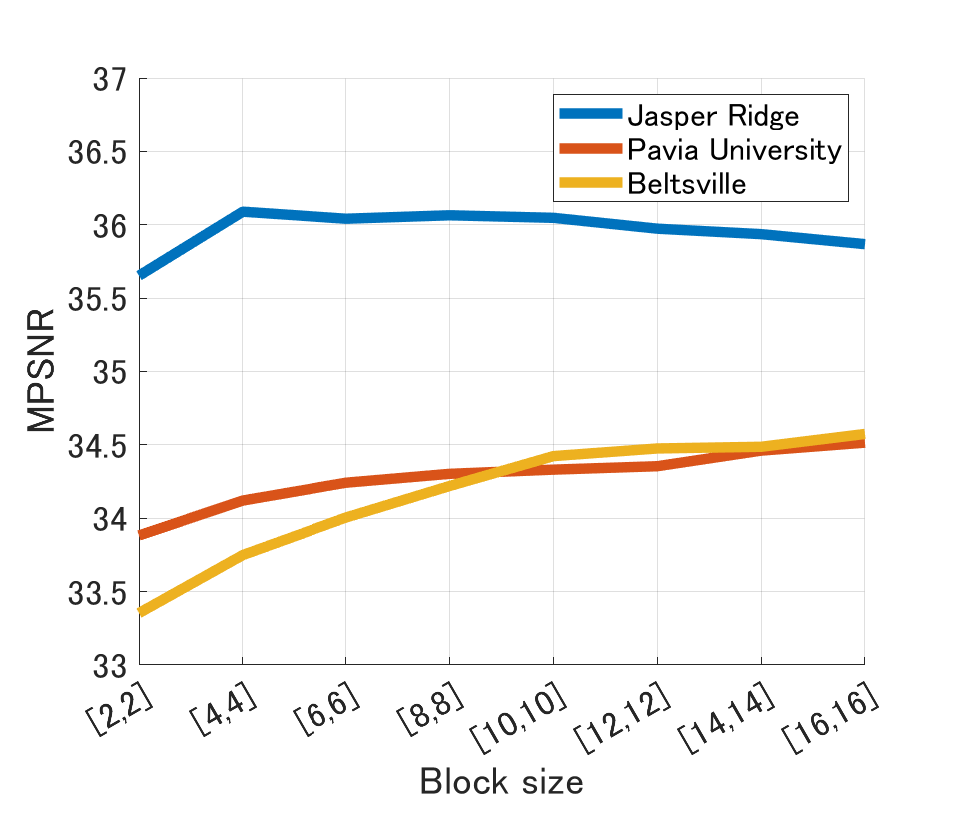
\includegraphics[width=\hsize]{./fig_Param_Anal/blocksize_mpsnr.eps}}
        \end{minipage}
        \begin{minipage}{0.240\hsize}
            \centerline{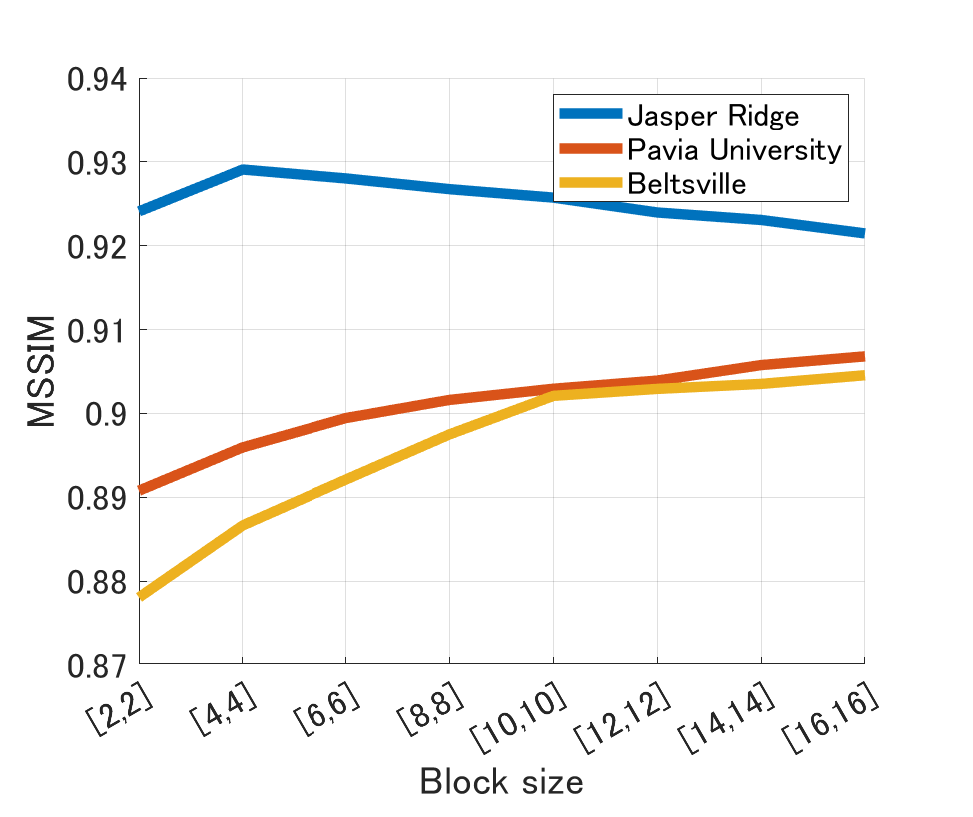
\includegraphics[width=\hsize]{./fig_Param_Anal/blocksize_mssim.eps}}
        \end{minipage}
        \begin{minipage}{0.240\hsize}
            \centerline{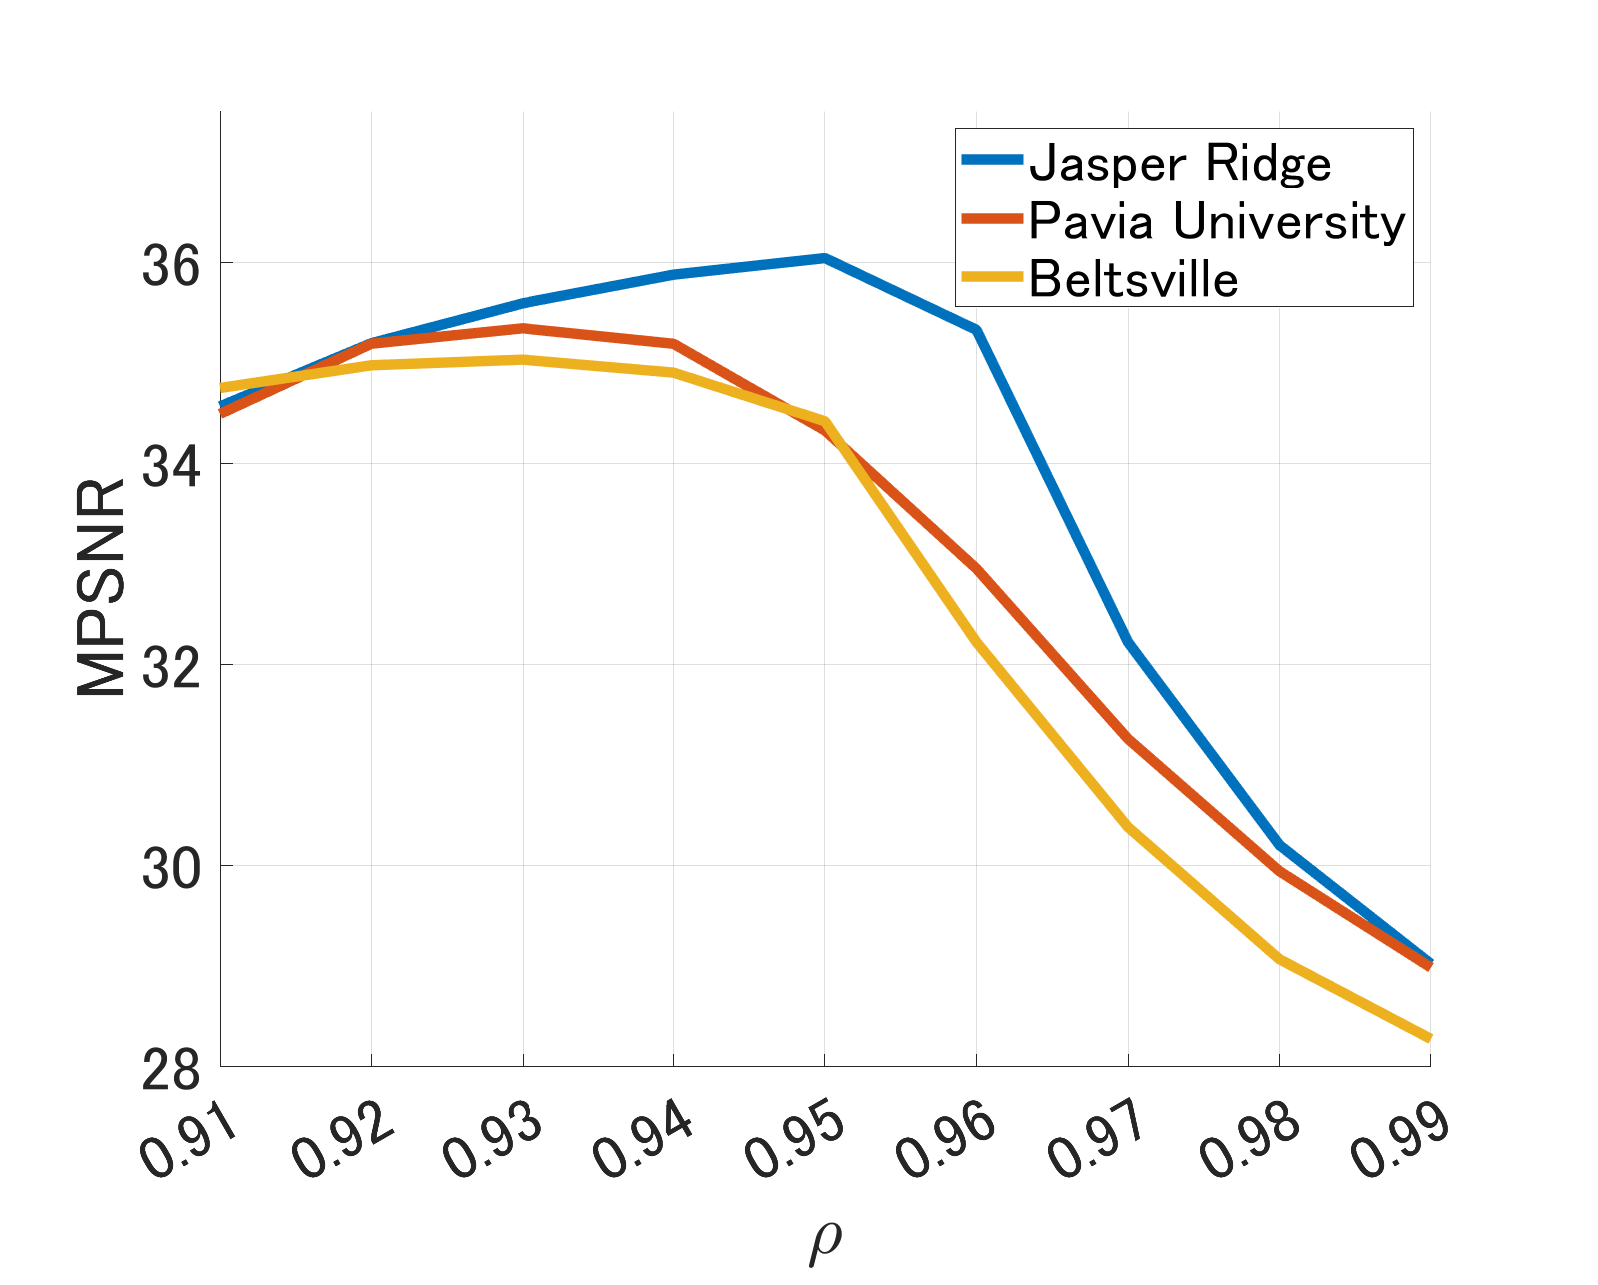
\includegraphics[width=\hsize]{./fig_Param_Anal/rho_mpsnr.eps}}
        \end{minipage}
        \begin{minipage}{0.240\hsize}
            \centerline{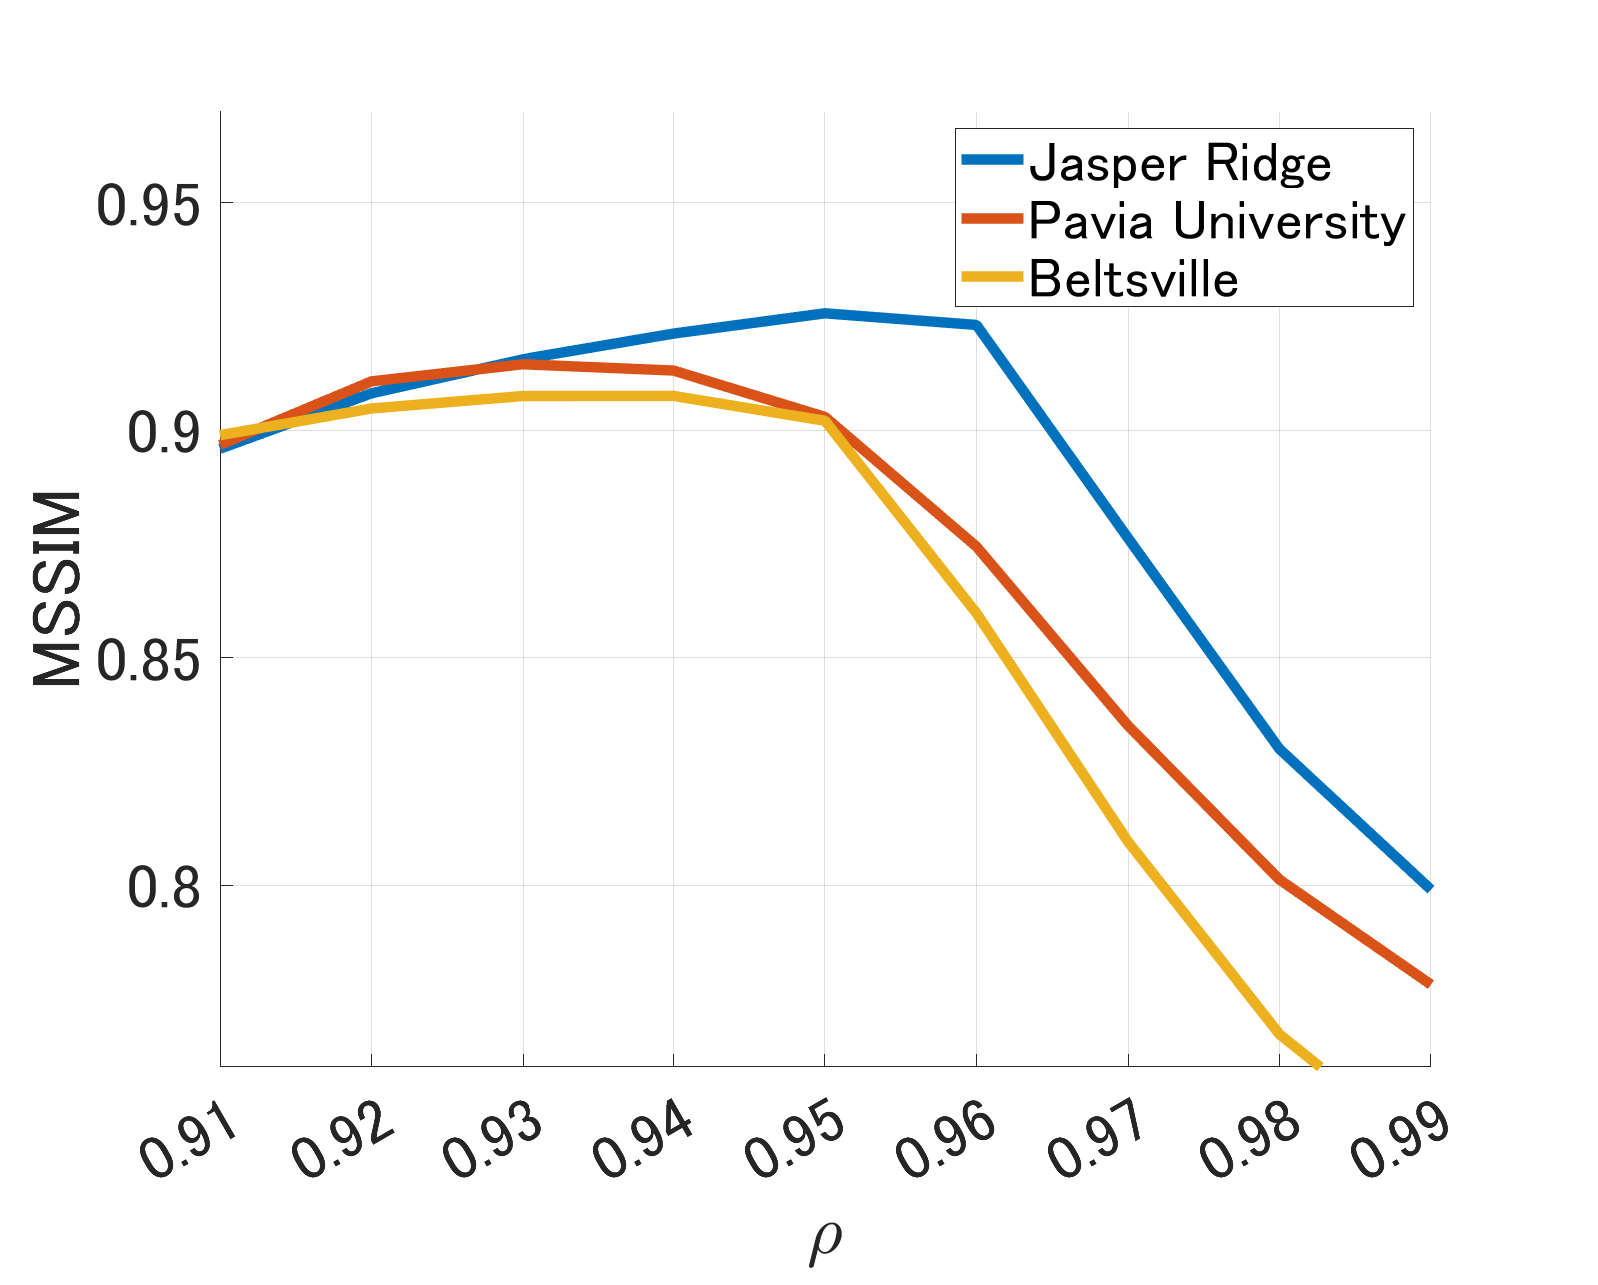
\includegraphics[width=\hsize]{./fig_Param_Anal/rho_mssim.eps}}
        \end{minipage}

        \begin{minipage}{0.240\hsize}
            \centerline{\small{(a)}}
		\end{minipage}
		\begin{minipage}{0.240\hsize}
			\centerline{\small{(b)}}
		\end{minipage}
		\begin{minipage}{0.240\hsize}
			\centerline{\small{(c)}}
		\end{minipage}
		\begin{minipage}{0.240\hsize}
			\centerline{\small{(d)}}
		\end{minipage}
    \end{center}
	
    \vspace{-3mm}
    \caption{Analysis of parameters in the proposed method: block size and $\ParamsRadius$. (a): MPSNR versus block size. (b): MSSIM versus block size. (c): MPSNR versus $\ParamsRadius$. (d): MSSIM versus $\ParamsRadius$. }
    \label{fig:Param_Anal}
\end{figure*}